\chapter{Anforderungen an das System}
\label{chap:systemanforderungen}

Im Folgenden werden die Anforderungen an das System definiert. Funktionale und nichtfunktionale Anforderungen werden in schriftlicher Form festgelegt, eine tabellarische Übersicht findet sich im Anhang (Abschnitt \ref{subsec:af-tabelle}). Die erforderlichen und erwünschten Funktionalitäten werden dabei auch durch Use-Case-Diagramme beschrieben. In diesem Kapitel soll die Frage beantwortet werden, was ein System leisten muss, damit es die in der Analyse (Kapitel \ref{chap:analyse}) beschriebenen Vorgaben erfüllt.

\section{Funktionale Anforderungen}
\label{sec:funktionale-af}

\subsection{Muss-Kriterien}
\label{subsec:muss}

 
Abbildung \ref{fig:usecasediagramm-muss-editor} zeigt ein Use-Case-Diagramm für die in den Muss-Kriterien definierten Anforderungen an die Outline-Verwaltung und den Gliederungseditor. In Abbildung \ref{fig:usecasediagramm-muss-repl} finden sich die Anforderungen an Replikation und Konfliktbehandlung. Der im Rahmen dieser Arbeit entwickelte Prototyp soll folgenden Anforderungen in jedem Fall entsprechen. Nur dann kann von einer erfolgreichen Umsetzung der Aufgabenstellung gesprochen werden. 

\medskip
\begin{figure}[ht] 
  \begin{center}
  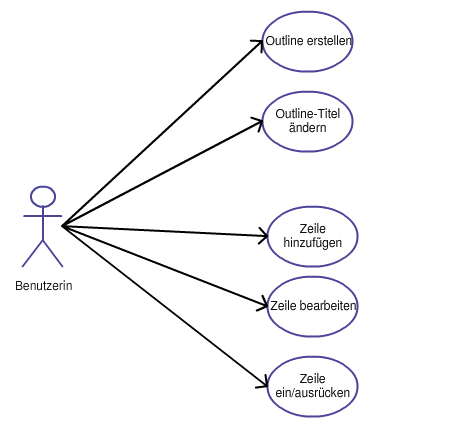
\includegraphics[width=0.6\textwidth]{grafik/usecasediagramm-muss-editor} 
  \end{center}
  \caption{Use-Case-Diagramm für die Muss-Kriterien, Outline-Verwaltung}
  \label{fig:usecasediagramm-muss-editor} 
\end{figure}

\medskip
\begin{figure}[ht] 
  \begin{center}
  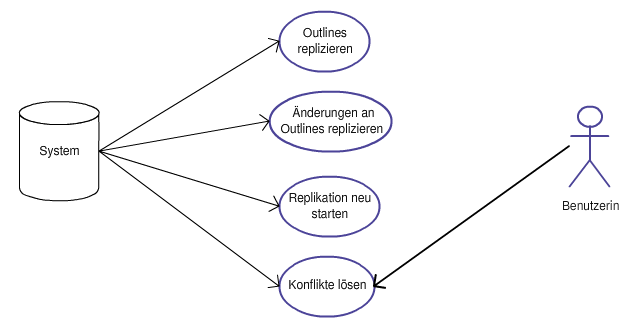
\includegraphics[width=\textwidth]{grafik/usecasediagramm-muss-repl} 
  \end{center}
  \caption{Use-Case-Diagramm für die Muss-Kriterien, Replikation}
  \label{fig:usecasediagramm-muss-repl} 
\end{figure}

\subsubsection{Outline-Verwaltung}

Der Benutzer muss eine beliebige Anzahl von Outlines erstellen können (\textbf{FA100}). Die Outlines müssen übersichtlich dargestellt werden und einen veränderbaren Titel haben (\textbf{FA101}). 

\subsubsection{Gliederungseditor}
\label{subsec:gliederungseditor}

Der Gliederungseditor muss das Look \& Feel eines Texteditors mit einer beliebigen Anzahl von Zeilen haben (\textbf{FA200}). Zwischen den Zeilen muss mit den üblichen Tasten/Tasten-Kombinationen navigiert werden können (\textbf{FA201}). Es muss möglich sein, den Inhalt der Zeilen zu bearbeiten (\textbf{FA202}). Beim Verlassen einer Zeile wird diese automatisch gespeichert (\textbf{FA203}). Wird das Fenster geschlossen, während eine Zeile editiert wird, muss diese automatisch gespeichert werden. Alternativ kann der Benutzer auch vor dem Schließen des Fensters darauf hingewiesen werden, dass Datenverlust zu befürchten ist (\textbf{FA206}).

Die Zeilen müssen ein- und wieder ausrückbar sein, um eine hierarchische Abbildung zu ermöglichen (\textbf{FA204}). Das Ein- bzw. Ausrücken einer Zeile soll die unmittelbar darunter liegenden Zeilen mit tieferer Einrückung mitbewegen (\textbf{FA205}).

\subsubsection{Replikation}

Ist der Benutzer online oder wird nach einer Offline-Phase die Verbindung wiederhergestellt, müssen von ihm erstellte Outlines (\textbf{FA300}) und von ihm gemachte Änderungen an Outlines (\textbf{FA301}) sofort zum Server repliziert werden. 

Der Benutzer muss alle im System von anderen Benutzern erstellten Outlines (\textbf{FA302}) und deren Änderungen an Outlines (\textbf{FA303}) automatisch auf seinen Rechner repliziert bekommen, sofern oder sobald diese mit dem Server verbunden sind. Er muss über Änderungen benachrichtigt werden, sobald diese vorliegen (\textbf{FA304}). Dabei soll der Arbeitsfluss nicht unterbrochen werden.

Wird nach einer Offline-Phase die Verbindung wiederhergestellt, muss der Benutzer entweder darauf hingewiesen werden, dass Replikation jetzt wieder möglich ist, oder die Replikation muss automatisch gestartet werden (\textbf{FA305}).

\subsubsection{Konfliktbehandlung}

Von den Konflikten, die beim Replizieren entstehen können, soll mindestens eine Art vom System selbstständig gelöst werden (\textbf{FA400}). Mindestens eine Konfliktart soll der Benutzer manuell lösen können (\textbf{FA401}).

\subsection{Kann-Kriterien}
\label{subsec:kann}

Die in diesem Abschnitt aufgestellten Kriterien müssen nicht alle im Prototyp implementiert werden. Beim Design des Systems soll allerdings ihre spätere Umsetzbarkeit miteinbezogen werden.

Abbildung \ref{fig:usecasediagramm-kann-editor} zeigt ein Use-Case-Diagramm für die in den Kann-Kriterien definierten Anforderungen an die Outline-Verwaltung und den Gliederungseditor. In Abbildung \ref{fig:usecasediagramm-kann-repl} finden sich die Anforderungen an Replikation und Konfliktbehandlung.


\medskip
\begin{figure}[ht] 
  \begin{center}
  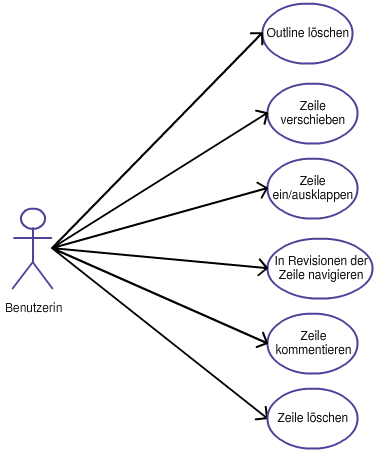
\includegraphics[width=0.6\textwidth]{grafik/usecasediagramm-kann-editor} 
  \end{center}
  \caption{Use-Case-Diagramm für die Kann-Kriterien, Outline-Verwaltung}
  \label{fig:usecasediagramm-kann-editor} 
\end{figure}

\medskip
\begin{figure}[ht] 
  \begin{center}
  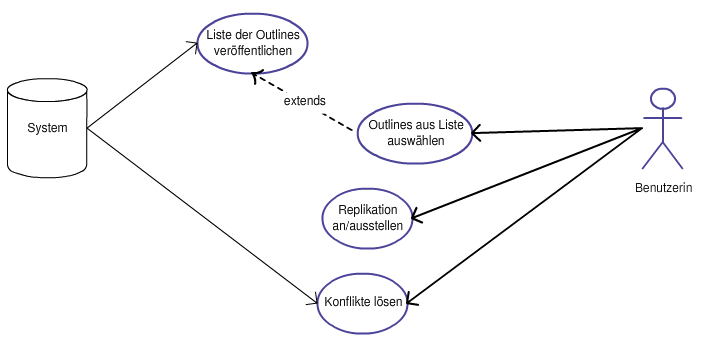
\includegraphics[width=\textwidth]{grafik/usecasediagramm-kann-repl} 
  \end{center}
  \caption{Use-Case-Diagramm für die Kann-Kriterien, Replikation}
  \label{fig:usecasediagramm-kann-repl} 
\end{figure}


\subsubsection{Outline-Verwaltung}

Outlines sollen gelöscht werden können (\textbf{FA102}).

\subsubsection{Gliederungseditor}

Die Zeilen sollen nach unten und oben verschoben werden können (\textbf{FA207}). Die Größe der Zeile soll sich automatisch an die Menge des Textes anpassen (\textbf{FA208}). Für eine verbesserte Übersichtlichkeit sollen die Zeilen ein- und ausklappbar sein (\textbf{FA209}). Die Information, welche Zeilen eingeklappt sind, soll nicht mitrepliziert, möglichst aber lokal gespeichert werden (\textbf{FA210}).

Die Revisionen einer Zeile sollen automatisch gespeichert werden (\textbf{FA211}). Zwischen den Revisionen soll gewechselt werden können (\textbf{FA212}). Es soll möglich sein, die einzelnen Zeilen mit Kommentaren zu versehen (\textbf{FA213}) und die Zeilen löschen (\textbf{FA214}).

\subsubsection{Replikation}

Die zur Verfügung stehenden Outlines sollen vom System veröffentlicht werden, so dass mit dem Server verbundene Benutzer auswählen können, welche einzelnen Outlines sie replizieren möchten (\textbf{FA306}).

Der Benutzer soll über eine Statusmeldung informiert werden, ob gerade eine Verbindung zum Server besteht oder nicht (\textbf{FA307}). Über das Interface soll es die Möglichkeit geben, Replikation an- und auszustellen (\textbf{FA308}). 

\subsubsection{Konfliktbehandlung}

Kombinationen aus unterschiedlichen Konfliktarten sollen vom System / vom Benutzer gelöst werden können (\textbf{FA402}). Konflikte, die zwischen mehr als zwei Repliken auftreten, sollen korrekt behandelt werden (\textbf{FA403}).

Es sollen möglichst viele Konflikte vom System selbstständig gelöst werden können (\textbf{FA404}). Die Oberfläche soll so entworfen sein, dass der Benutzer möglichst viele Konfliktarten manuell lösen kann (\textbf{FA405}).


\subsection{Abgrenzungs-Kriterien}

\subsubsection{Outline-Verwaltung}

Es wird keine Benutzerverwaltung und keine Zugriffsverwaltung für Outlines implementiert.

\subsubsection{Gliederungseditor}

Es werden keine Spalten implementiert. 

\subsubsection{Replikation}

Es wird keine Peer-to-Peer-Replikation geben.

\subsubsection{Konfliktbehandlung}

Das System wird nur für die Benutzung durch eine kleine Anzahl Benutzer optimiert sein. Bei Konflikten zwischen mehr als zwei kollidierenden Versionen ist eine verlässliche Konfliktbehandlung nicht gesichert.


\section{Nichtfunktionale Anforderungen}

\subsection{Einsatz}
\label{subsec:einsatz}

\subsubsection{Zielgruppe}

Benutzer des Systems müssen durchschnittliche Kenntnisse in der Bedienung eines Computers, insbesondere eines Webbrowsers haben. Des Weiteren müssen sie in der Lage sein, eine CouchDB-Instanz auf ihrem Rechner zu installieren und zu starten. Bei den Benutzern sollte ein Verständnis für die Vorteile und Grenzen der Einsatzmöglichkeiten des Systems vorhanden sein.

\subsubsection{Betriebsbedingungen}

Der Server für den Austausch der Outlines und der Updates muss stabil 24 Stunden am Tag und sieben Tage die Woche laufen, damit die Dienste jederzeit verfügbar sind. Um dies sicherzustellen, soll das Deployment mit dem Service Amazon Elastic Compute Cloud (Amazon EC2) vorgenommen werden. Für bessere Skalierbarkeit soll darüber hinaus das Clustering Framework CouchDB-Lounge eingesetzt werden.

Die Anwendung soll auf jedem Rechner bereitgestellt werden können, auf dem CouchDB installiert werden kann. Nähere Hinweise zu von CouchDB unterstützten Systemen finden sich in Abschnitt \ref{sec:installation}.

\subsection{Umgebung}

Um Lizenzgebühren zu vermeiden und das System an wechselnde Anforderungen anpassen zu können, soll es ausschließlich mit Open-Source Software umgesetzt werden. 


\subsubsection{Hardware}

Wenn die Couch-Instanz, die als Server dienen soll, nicht mit Amazon EC2, sondern auf einem eigenen Server bereitgestellt wird, muss dieser folgenden Mindestanforderungen genügen:

\begin{itemize}  
  \item[-] Intel-Prozessor mit Frequenz 3,0 Ghz
  \item[-] mind. 5 GB Festplatte 
  \item[-] 1 GB Hauptspeicher 
  \item[-] LAN-Anschluss Fast Ethernet 100 MBit
\end{itemize}


\subsubsection{Software}

Das System baut auf mehreren Softwarepaketen und Programmiersprachen auf. Die angegebenen Versionen sind Mindestanforderungen. Hinweise zur Installation finden sich in Abschnitt \ref{sec:installation}.

\begin{itemize}  
  \item[-] CouchDB 0.11.0
  \item[-] Spidermonkey 1.7
  \item[-] Erlang 5.6.5
  \item[-] ICU 3.0
  \item[-] cURL 7.18.0
  \item[-] Automake 1.6.3
  \item[-] Autoconf 2.59
\end{itemize}

Wenn die mitgelieferten Rake-Tasks für Deployment und Betrieb genutzt werden sollen, muss Ruby in der Version 1.8.6. oder größer installiert werden (s. Abschnitt \ref{subsec:hilfestellung}).

Hinweise für das Testsetup finden sich in Abschnitt \ref{sec:systemtest}.


\subsection{Benutzeroberfläche}
\label{subsec:gui-anf}

Für das System soll eine einfache und übersichtliche Web-Oberfläche gestaltet werden. Die Aktivierung von JavaScript kann vorausgesetzt werden. Die Oberfläche soll mindestens im Browser Firefox in der Mindestversion 3.5 vollständig funktionieren. Die Verzögerung zwischen Eingabe auf der Weboberfläche und Eintreten der gewünschten Funktionen sollte möglichst weniger als eine Sekunde, in keinem Fall aber mehr als vier Sekunden betragen. Diese Zeitspanne wird in einer Studie als noch tolerierbare Wartezeit auf Antwort in zwischenmenschlichen Gesprächen bzw. in Telefonsystemen bezeichnet \citelit[S. 267 bzw. 270]{response:miller}. Jakob Nielsen überträgt diese Zeitspanne auf Interaktionszeiten mit Webapplikationen \citelit[Kap. 5.5]{nielsen:response}.

Abbildung \ref{fig:interface-mockup-list} zeigt ein Mockup für die Struktur der Seite mit der Outline-Übersicht. Abbildung \ref{fig:interface-mockup} zeigt den Aufbau der Seite, die den Gliederungseditor enthält.


\medskip
\begin{figure}[ht] 
  \begin{center}
  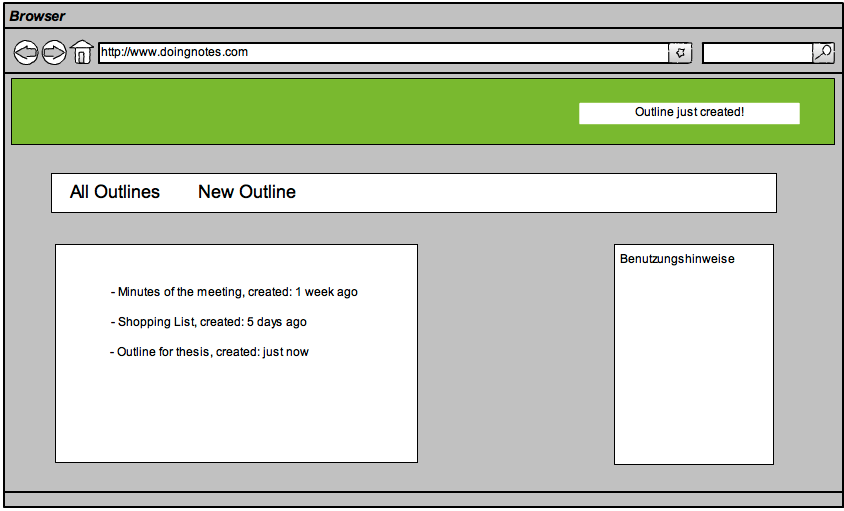
\includegraphics[width=\textwidth]{grafik/user-interface-mockup-list} 
  \end{center}
  \caption{Struktur der Web-Oberfläche: Outline-Übersicht}
  \label{fig:interface-mockup-list} 
\end{figure}

\medskip
\begin{figure}[ht] 
  \begin{center}
  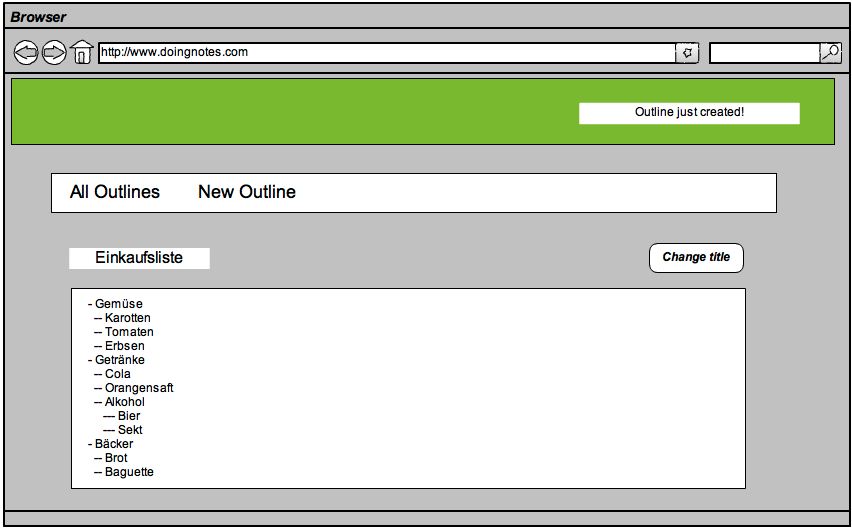
\includegraphics[width=\textwidth]{grafik/user-interface-mockup} 
  \end{center}
  \caption{Struktur der Web-Oberfläche: Outline-Einzelansicht}
  \label{fig:interface-mockup} 
\end{figure}


\subsection{Qualitätsziele}

Die Qualität des erstellten Systems ist ein weiteres wichtiges Ziel. Die qualitativen Anforderungen sind folgende:

\begin{itemize}  
  \item Erweiterbarkeit durch offene Architektur
  \item Portabilität durch geringe Hardware- und Software-Anforderungen
  \item Hohe Softwarequalität durch möglichst flächendeckende Testabdeckung
  \item Design und Programmierung orientiert an sprach- und frameworkspezifischen Standards
  \item Implementierung nach der MVC-Architektur: Trennung zwischen Oberfläche / Anwendungslogik / Datenhaltung
  \item Möglichst wartbarer, deshalb einfacher und redundanzfreier Code
  \item Einhaltung von Usability- und Accessability-Guidelines bei der Oberfläche
  \item Geringe Ladezeiten der Anwendung im Browser, deshalb möglichst wenig Abhängigkeit von externen Frameworks
\end{itemize}

